%%%%%%%%%%%%%%%%%%%%%%%%%%%%%%%%%%%%%%%%%%%%%%%%%%%%%%%%%%%%%%%%%%%%%%%%%%%%%%%%
% Author : [Jachym] [Dolezal], Tomas Polasek (template)
% Description : Seventh exercise in the Introduction to Game Development course.
%   It deals with the creation of a Game Design Document, presenting a short 
%   pitch for a potential game project.
%%%%%%%%%%%%%%%%%%%%%%%%%%%%%%%%%%%%%%%%%%%%%%%%%%%%%%%%%%%%%%%%%%%%%%%%%%%%%%%%

\documentclass[a4paper,10pt,english]{article}

\usepackage[left=2.50cm,right=2.50cm,top=1.50cm,bottom=2.50cm]{geometry}
\usepackage[utf8]{inputenc}

% Hyper-Text References
\usepackage{hyperref}
\hypersetup{colorlinks=true, urlcolor=blue}

% Drawing Images and Graphs
\usepackage{tikz}
\usepackage{pgfplots}

% Page Utilities
\usepackage{graphicx}

% Image Sub-Captions
\usepackage{subcaption}

\newcommand{\ph}[1]{\textit{[#1]}}

\title{%
Game Pitch Document%
}
\author{%
Jáchym Doležal (xdolez0c)%
}
\date{}

\begin{document}

\maketitle
\thispagestyle{empty}

{%
\large

\begin{itemize}

\item[] \textbf{Title:} Duel of The Bards

\item[] \textbf{Genre:} Music Rhythm \& RTS

\item[] \textbf{Style:} 3D from bird's eye perspective, Cartoon style
\item[] \textbf{Platform:} PC 

\item[] \textbf{Market:} people of all ages interested in strategy, RTS, and rhythm games.

\item[] \textbf{Elevator Pitch:}

\end{itemize}

}

\section*{\centering The Pitch}

Duel of The Bards: A groundbreaking fusion of RTS and rhythm games. Players must finetune their strategy, commanding armies while simultaneously honing their rhythmic skills to spawn new troops. This game challenges players to a dual test of tactical prowess and rhythm-based agility, offering an unparalleled, exciting battle experience.

\subsection*{Introduction}

The main premise of Battle of the Bards is to connect two distinct genres, RTS and music rhythm, in a new and interesting way. The aim is to take the most intriguing and entertaining aspects of both genres and experience them together. Players will have to manage their troops across the map strategically and react to the opponent's attack together with managing their army. By training new troops players will have to concentrate on the music played while thinking of new moves they have to do on the map. There will be three types of troops they can train; Archers, Swordsman and Cavalry. The game will also have an economy of points and gold gained from capture points players can capture across the map. 

\subsection*{Background}

The RTS genre was trendy back then. Nowadays there are still a lot of players playing RTS and there are a lot of indie strategic games. There is still a demand for RTS games, but this genre is difficult to get in for new people because it requires skills most of the other games don't. To excel and be good at RTS people have to have fast decision-making and be able to play fast, using macros for building and managing armies effectively. That's what makes it exciting when combined with Music rhythm. Music rhythm games require precise fast and precise timing which is the same as for RTS. There are the more classical rhythm games OSU or A Dance of Fire and Ice which inspired roguelike rhythm games such as BPM (Bullets Per Minute) or Crypt of the NecroDancer. Battle of the Bards would be challenging for both fan bases of these genres and it would combine these two fanbases which would have the potential for success.

\subsection*{Setting}
The game is set in the Scandinavian lands of Clans where leaders are bards with magic instruments that can summon their troops with motivation for battle. Battles between the clans are essentially music battles between the two Leaders where the winner gets all. The plot and setting are not the most important aspects of the game, but there could be a campaign of some sort or additional lore for the clans that would help to immerse players.

\subsection*{Features}
What are the main selling points of your game? Think about the target market and market values of
your game. What makes it unique among other, already existing games? Why would players want to
play your game instead of some other? You can use a bullet point list or combine it with a value graph.

The most interesting aspect of this game is the unique mixture of genres that require new skills for the gameplay. It takes the aspects for precision and fast decision-making needed in both genres and makes them more important with its combination. Furthermore, the fact that this game can bring new people into the genres and combine player bases of the two genres makes it interesting from the market perspective because it can have a large number of players. This section will further describe the main aspects of the game.

\subsubsection*{Types of troops}
\begin{itemize}
    \item Archers - unit specialized on long-range, is stronger against swordsman and is faster than swordsman.
    \item Cavalry - Fastest unit and has bonus against archers.
    \item Swordsman - This unit has good armour and has a bonus against cavalry.
\end{itemize}
\subsubsection*{Spawning of troops}

Each troop type is created by playing different kinds of music with specific features. Spawning the troops costs the stamina of the players which can be refilled over time. The speed and capacity of regaining stamina can be upgraded. While playing, the movement speed of the bards is decreased and spawns the particular troops by their side. After they cancel the song or they fail too many notes in a row they stop playing and receive a cooldown for the troops spawning.

\subsubsection*{The winning conditions}

\begin{itemize}
    \item One of the bards reaches the maximum points first
    \item The first that kills the other Bard.
    \item The one who has the most points after the time goes off.
\end{itemize}

\subsubsection*{Map}

The mas has spawn points of the Bards. There are capture points that can be captured by troops but must be claimed by Bard to receive points from them. The capture points can be upgraded by gold too. The first upgrade creates an outpost in the place of the point with more health. The second upgrade creates a stone tower that shoots at close enemies. Gold can be also used by Bards to upgrade themselves and their troops. Besides the game points capture points also increase gold gain. 

\subsection*{Genre}

The main genre is RTS with its classical aspects, where, in our case, two players battle against each other with their created troops and fight over resources which help them to gather a greater army. Each unit has multiple soldiers where they are controlled and each of them has unique stats of HP, damage, etc. The secondary genre supports the main genre by making it more interesting. The traditional mechanic where the troops are created by a certain structure or bought and trained over time, Battle of the Bards replaces this process with a minigame similar to music rhythm games such as Guitar Hero. Hence, both of these genres are present. 

\subsection*{Platform}
This game will be aimed mainly on PC. The easiest platforms would be Linux and Windows. If possible console development could be possible, but RTS is not that popular on these devices. 
  

\subsection*{Style}

The game would have a cartoon style similar to games such as League of Legends or Dota. This style also fits with the rhythm mechanic which would fit to a more cartoonish game style rather than realistic and dark styles. I created some examples of concept art for my troops and Bard or instruments that they could be playing using DALL-E, so these are not my work. 


\begin{figure}[h]

\centering

\begin{subfigure}{0.29\linewidth}
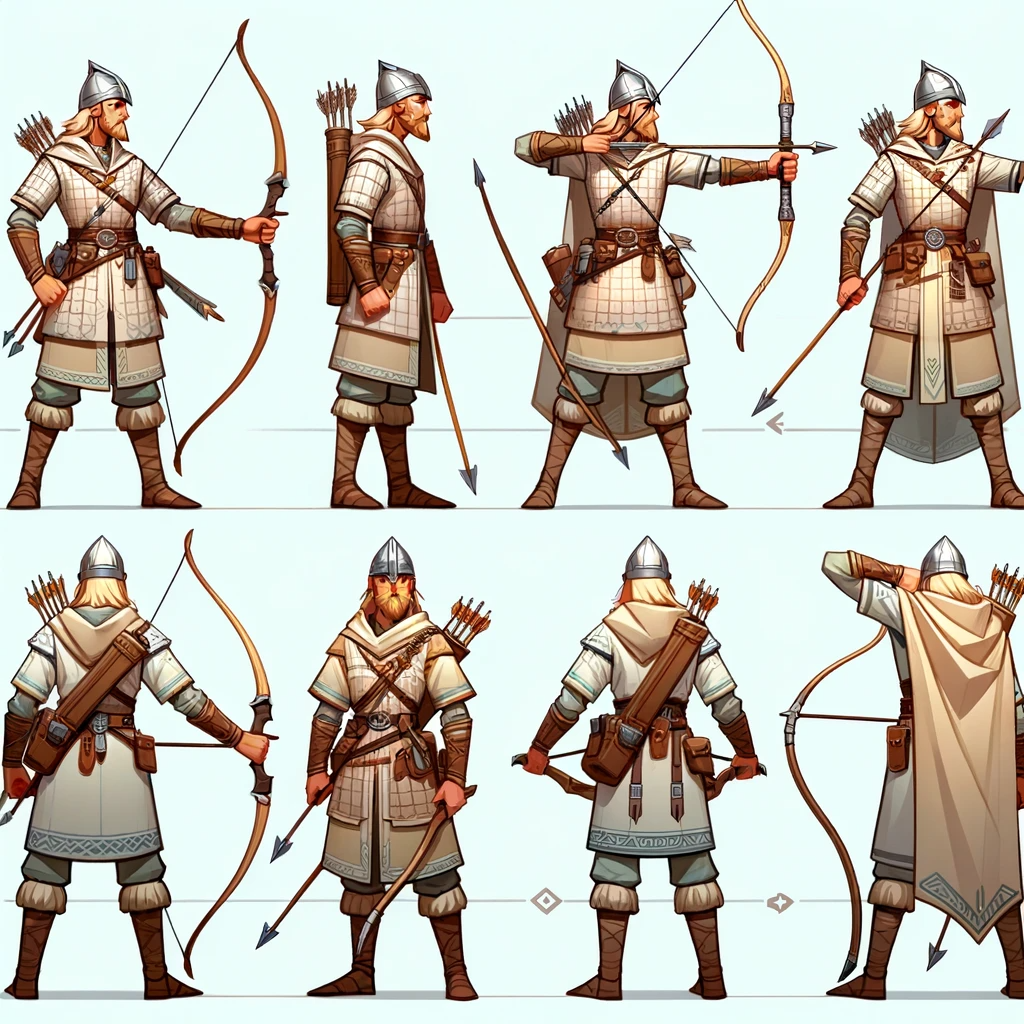
\includegraphics[width=\linewidth]{archers.png}
\captionof{figure}{Concept art of archers}
\label{Fig:Style1A}
\end{subfigure}\hfill
%
\begin{subfigure}{0.29\linewidth}
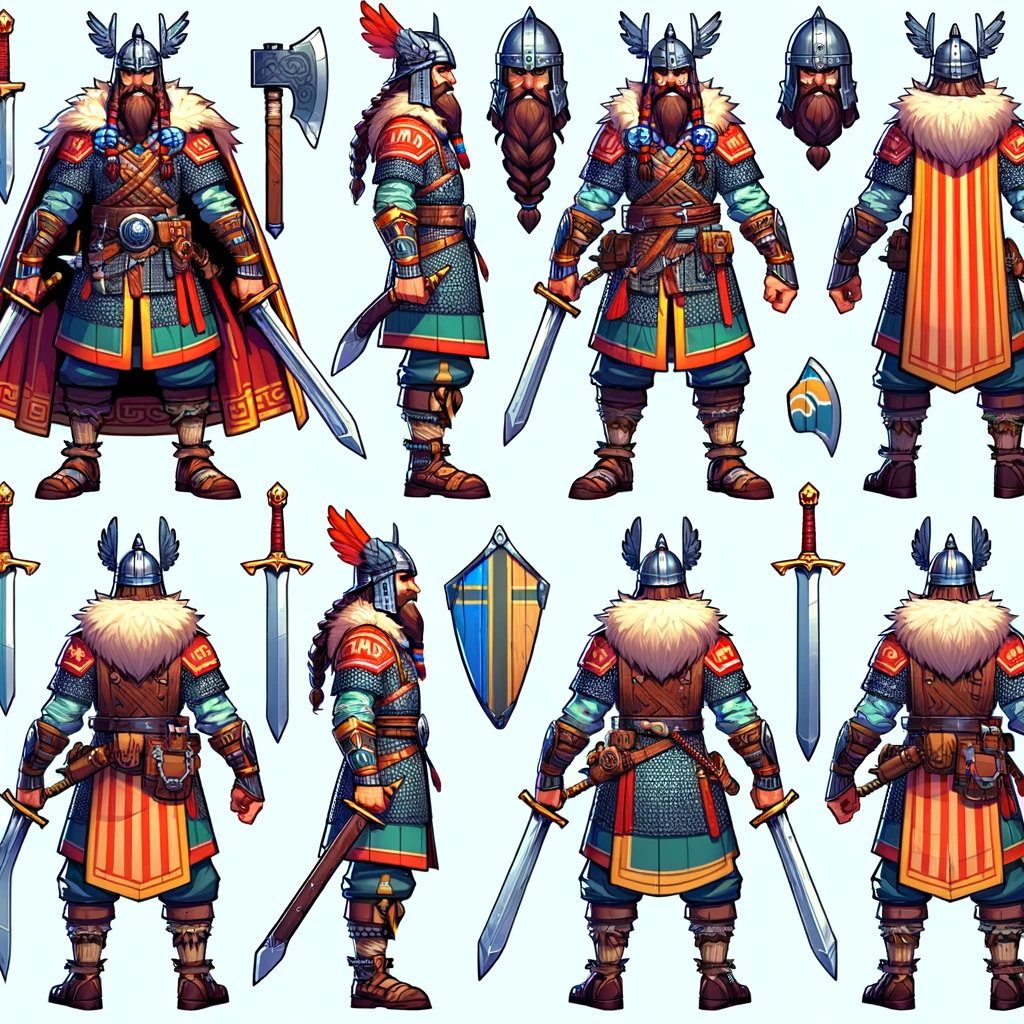
\includegraphics[width=\linewidth]{swordsman.png}
\captionof{figure}{Concept art of swordsman}
\label{Fig:Style1B}
\end{subfigure}\hfill
%
\begin{subfigure}{0.29\linewidth}
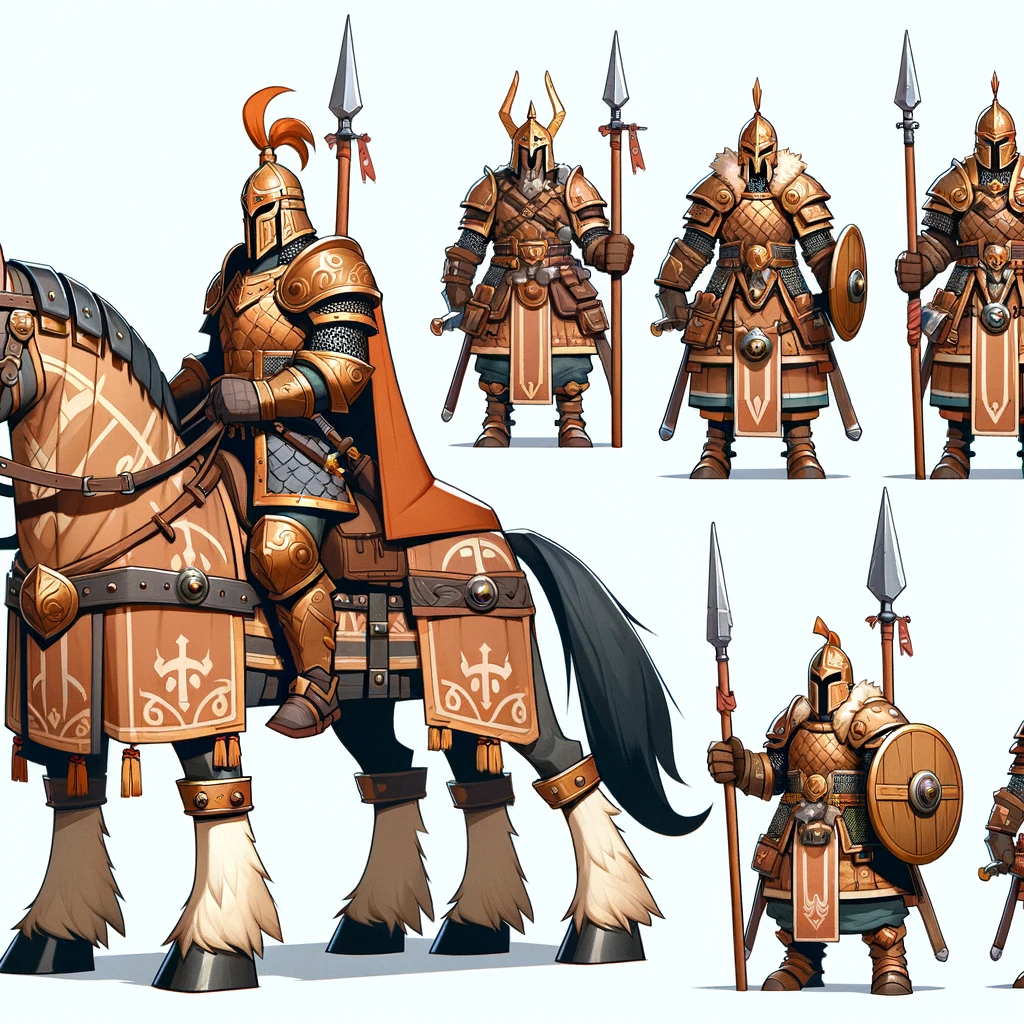
\includegraphics[width=\linewidth]{cavalry.png}
\captionof{figure}{Concept art of Cavalry}
\label{Fig:Style1C}
\end{subfigure}

\end{figure}

\begin{figure}[h]

\centering

\begin{subfigure}{0.29\linewidth}
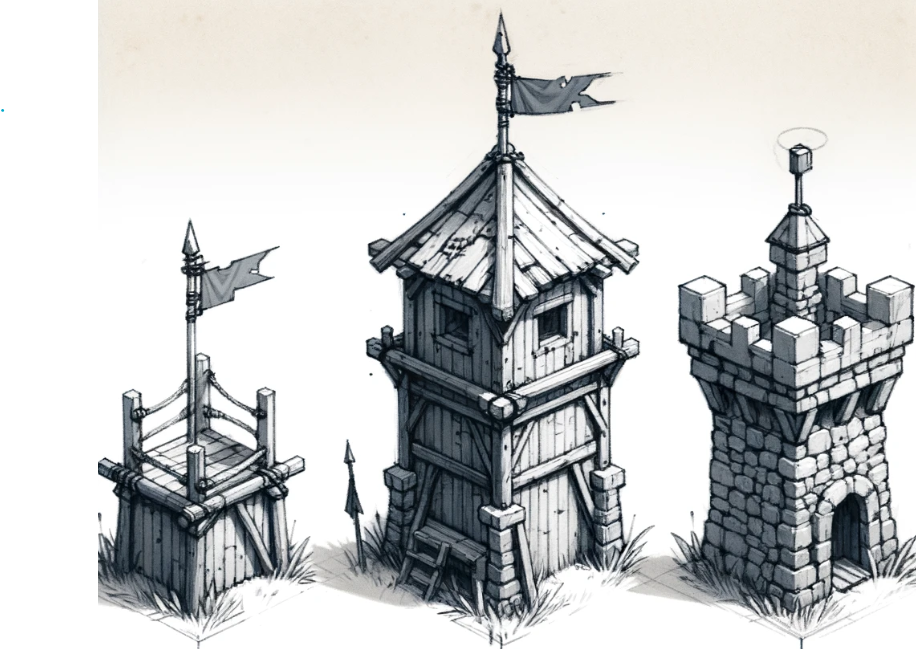
\includegraphics[width=1.2\linewidth]{capturepoint.png}
\captionof{figure}{Concept art of capture point}
\label{Fig:Style1A}
\end{subfigure}\hfill
%
\begin{subfigure}{0.29\linewidth}
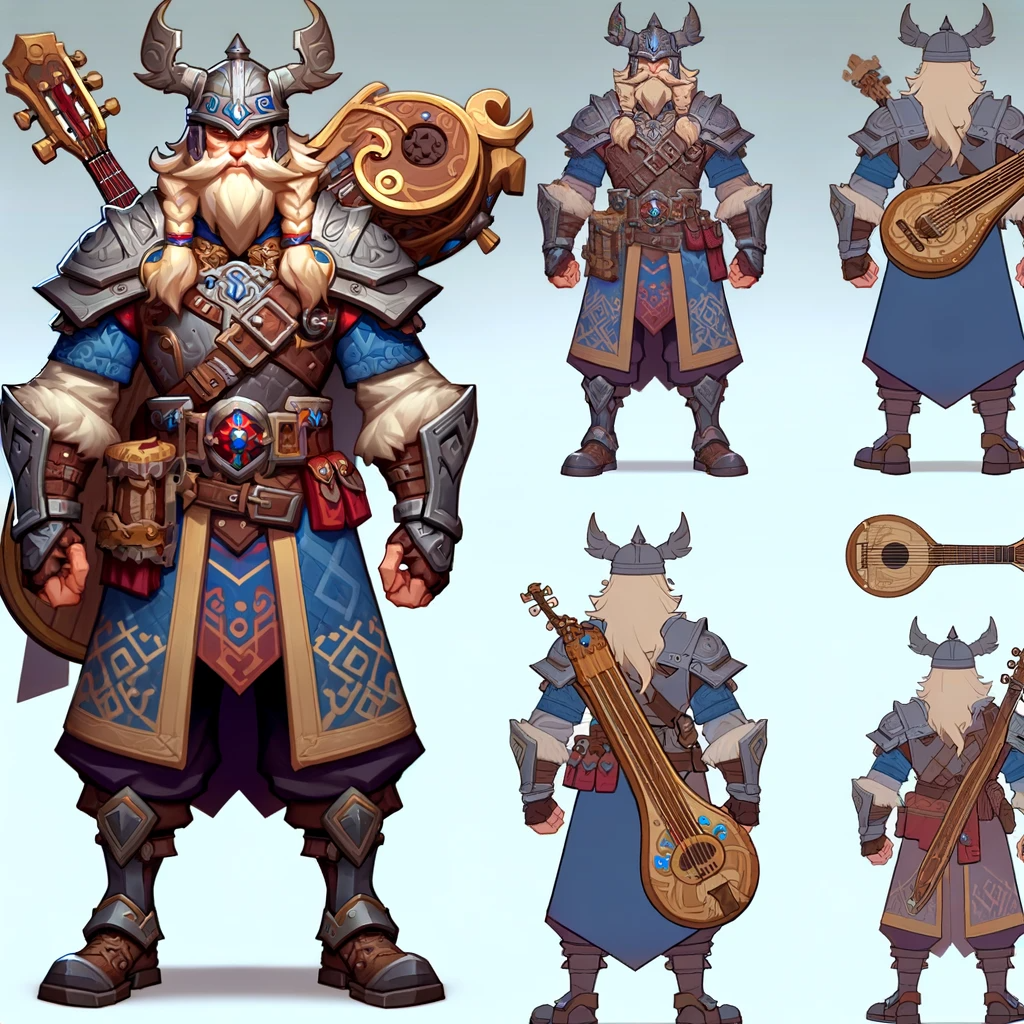
\includegraphics[width=\linewidth]{bard main.png}
\captionof{figure}{Concept art of Bard}
\label{Fig:Style1B}
\end{subfigure}\hfill
\end{figure}

\begin{figure}[h]
    \centering
 \rotatebox{90}{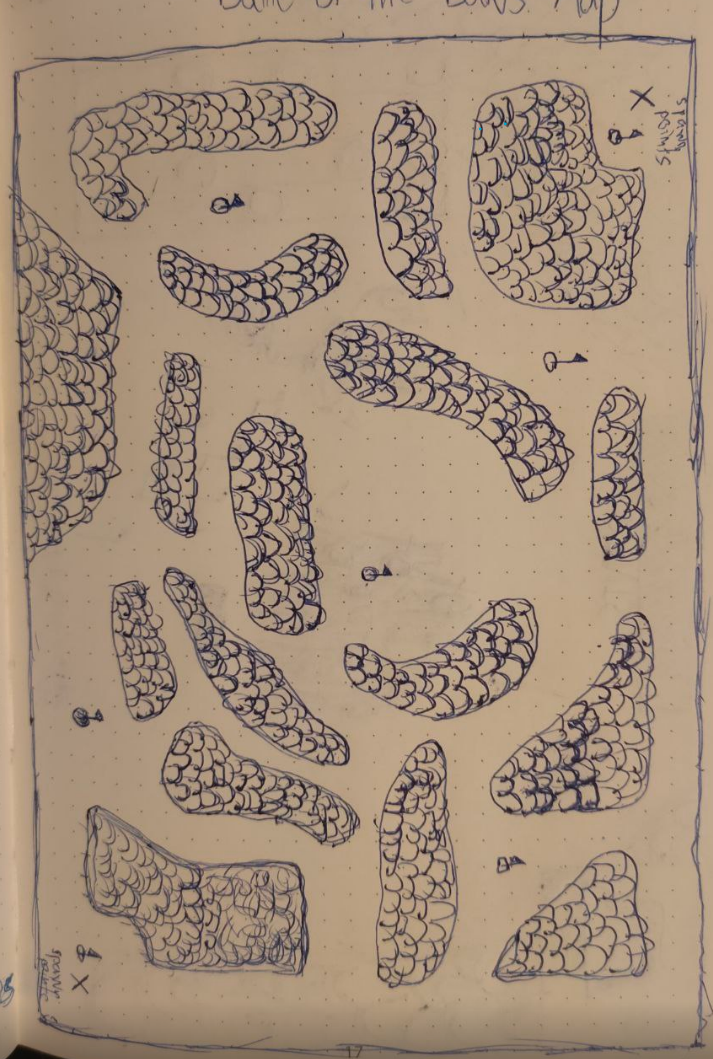
\includegraphics[width=0.45\textwidth]{map.png}}
    \caption{Concept art of the Map}
    \label{fig:yourlabel}
\end{figure}

\end{document}
